
%% bare_jrnl_compsoc.tex
%% V1.4a
%% 2014/09/17
%% by Michael Shell
%% See:
%% http://www.michaelshell.org/
%% for current contact information.
%%
%% This is a skeleton file demonstrating the use of IEEEtran.cls
%% (requires IEEEtran.cls version 1.8a or later) with an IEEE
%% Computer Society journal paper.
%%
%% Support sites:
%% http://www.michaelshell.org/tex/ieeetran/
%% http://www.ctan.org/tex-archive/macros/latex/contrib/IEEEtran/
%% and
%% http://www.ieee.org/

%%*************************************************************************
%% Legal Notice:
%% This code is offered as-is without any warranty either expressed or
%% implied; without even the implied warranty of MERCHANTABILITY or
%% FITNESS FOR A PARTICULAR PURPOSE! 
%% User assumes all risk.
%% In no event shall IEEE or any contributor to this code be liable for
%% any damages or losses, including, but not limited to, incidental,
%% consequential, or any other damages, resulting from the use or misuse
%% of any information contained here.
%%
%% All comments are the opinions of their respective authors and are not
%% necessarily endorsed by the IEEE.
%%
%% This work is distributed under the LaTeX Project Public License (LPPL)
%% ( http://www.latex-project.org/ ) version 1.3, and may be freely used,
%% distributed and modified. A copy of the LPPL, version 1.3, is included
%% in the base LaTeX documentation of all distributions of LaTeX released
%% 2003/12/01 or later.
%% Retain all contribution notices and credits.
%% ** Modified files should be clearly indicated as such, including  **
%% ** renaming them and changing author support contact information. **
%%
%% File list of work: IEEEtran.cls, IEEEtran_HOWTO.pdf, bare_adv.tex,
%%                    bare_conf.tex, bare_jrnl.tex, bare_conf_compsoc.tex,
%%                    bare_jrnl_compsoc.tex, bare_jrnl_transmag.tex
%%*************************************************************************


% *** Authors should verify (and, if needed, correct) their LaTeX system  ***
% *** with the testflow diagnostic prior to trusting their LaTeX platform ***
% *** with production work. IEEE's font choices and paper sizes can       ***
% *** trigger bugs that do not appear when using other class files.       ***                          ***
% The testflow support page is at:
% http://www.michaelshell.org/tex/testflow/


\documentclass[10pt,conference,onecolumn,compsoc]{IEEEtran}


\usepackage{hyperref}
\usepackage{enumitem}
\setlist[itemize]{leftmargin=3 cm}
\setlist[enumerate]{leftmargin=3cm}



% *** CITATION PACKAGES ***
%
\ifCLASSOPTIONcompsoc
  % IEEE Computer Society needs nocompress option
  % requires cite.sty v4.0 or later (November 2003)
  \usepackage[nocompress]{cite}
\else
  % normal IEEE
  \usepackage{cite}
\fi
% cite.sty was written by Donald Arseneau
% V1.6 and later of IEEEtran pre-defines the format of the cite.sty package
% \cite{} output to follow that of IEEE. Loading the cite package will
% result in citation numbers being automatically sorted and properly
% "compressed/ranged". e.g., [1], [9], [2], [7], [5], [6] without using
% cite.sty will become [1], [2], [5]--[7], [9] using cite.sty. cite.sty's
% \cite will automatically add leading space, if needed. Use cite.sty's
% noadjust option (cite.sty V3.8 and later) if you want to turn this off
% such as if a citation ever needs to be enclosed in parenthesis.
% cite.sty is already installed on most LaTeX systems. Be sure and use
% version 5.0 (2009-03-20) and later if using hyperref.sty.
% The latest version can be obtained at:
% http://www.ctan.org/tex-archive/macros/latex/contrib/cite/
% The documentation is contained in the cite.sty file itself.



% *** GRAPHICS RELATED PACKAGES ***
%
\ifCLASSINFOpdf
   \usepackage[pdftex]{graphicx}
 
\else
 
\fi
% graphicx was written by David Carlisle and Sebastian Rahtz. It is
% required if you want graphics, photos, etc. graphicx.sty is already
% installed on most LaTeX systems. The latest version and documentation
% can be obtained at: 
% http://www.ctan.org/tex-archive/macros/latex/required/graphics/
% Another good source of documentation is "Using Imported Graphics in
% LaTeX2e" by Keith Reckdahl which can be found at:
% http://www.ctan.org/tex-archive/info/epslatex/
%
% latex, and pdflatex in dvi mode, support graphics in encapsulated
% postscript (.eps) format. pdflatex in pdf mode supports graphics
% in .pdf, .jpeg, .png and .mps (metapost) formats. Users should ensure
% that all non-photo figures use a vector format (.eps, .pdf, .mps) and
% not a bitmapped formats (.jpeg, .png). IEEE frowns on bitmapped formats
% which can result in "jaggedy"/blurry rendering of lines and letters as
% well as large increases in file sizes.
%
% You can find documentation about the pdfTeX application at:
% http://www.tug.org/applications/pdftex









% *** PDF, URL AND HYPERLINK PACKAGES ***
%
\usepackage{url}
% url.sty was written by Donald Arseneau. It provides better support for
% handling and breaking URLs. url.sty is already installed on most LaTeX
% systems. The latest version and documentation can be obtained at:
% http://www.ctan.org/tex-archive/macros/latex/contrib/url/
% Basically, \url{my_url_here}.




\begin{document}

\title{Calender App
%
%

% received ..."  text while in non-compsoc journals this is reversed. Sigh.

\author{Jeremy Gordon\\ Kyle Byassee% <-this % stops a space
}
}
\IEEEtitleabstractindextext{%
\begin{abstract}
Our group project is a calender application. Some of the functions are notifying the user of events and customizing the user experience with pictures. The target audience are users that want more freedom from their calendar application. 
\end{abstract}
}

% make the title area
\maketitle
\IEEEdisplaynontitleabstractindextext
\IEEEpeerreviewmaketitle

\section{Introduction}
Our group project is a calender application, it is a C\# WPF application. Some of the functions are notifying the user of events and customizing the user experience with pictures. We are targeting individuals who want the ability to customize, export, import and set specific day/month/year/time notifications. 
We want to give the user a calendar application that better than what is offered currently from calendly or canvas.

\subsection{Background}
We decided on this project because we do not have much experience in C\#. We also felt we could improve on the traditional calender application providing additional freedom and features. Providing features like viewing historic information and customizing backgrounds with user pictures. A calender application sounded like a project that could be a fun, challenging and worthwhile semester long project.

\subsection{Impacts}
The project is geared towards a general audience. Our application is appealing to that audience because of the ability to customize the look of the applications background and set custom notifications. It may have a small, but positive effect on the end user by helping to manage and organize life events.

\subsection{Challenges}
The layout of the GUI seems daunting since some months have more days than others. We plan to take inspiration from the numerous calender applications that are already in the wild. While also improving on the GUI layout making it more user friendly and intuitive.

One challenge we encountered early on was changing the background of the calendar. We eventually overcame that challenge by searching online forums and other sources of information. Another challenge was setting the dates for notifications. The GUI is a still a challenge to make it appealing and modern looking.

\section{Scope}
The app will display the current date and time when first opened. Let the user change the date and set a notification on that date at a specific time. The user is be able to set the background of the app to a designated picture format. 

%\subsubsection{Stretch-Goals}
The stretch goals are to export a user profile to be imported later into the same or different calender application and adding weather to be displayed in the GUI of the application.

\subsection{Requirements}
The functional and non-functional requirements were gathered based upon what the program would need to be considered complete. We decided early on that the functional requirements should put our calendar on functional parity with other existing calendars. So we minimally came up with the following list.

\subsubsection{Functional}
\begin{itemize}
\item User needs to be able to specify a specific day/month/year to add a notification.
\item User can change background of the calendar with a picture.
\item User can change and navigate through the month, year and day.
\item User can cancel or modify an existing notification.
\end{itemize}

\subsubsection{Non-Functional}
\begin{itemize}
%\item User saved notifications should be encoded to protect user data.
\item The calendar can run in the background.
\end{itemize}

\subsection{Use Cases}
%\ref{tab:useCaseIndex}

\begin{table}
\centering
\begin{tabular}{|c|c|c|c|c|}
\hline
Use Case ID & Use Case Name & Primary Actor & Complexity & Priority\\
\hline
1 & Set a notification & User & Med & 1\\
\hline
2 & remove or change a set notification & User & Med & 1\\
\hline
3 & Change calender background & User & Low & 1\\
\hline
4 & View historic information & User & Low & 1\\
\hline
\end{tabular}
\caption{Sample use case table}
\label{tab:useCaseIndex}
\end{table}

\begin{itemize}
\item[Use Case Number:] 1
\item[Use Case Name:] Set a notification
\item[Description:] The user has a specific date and time they with for a notification to appear on. The user navigates to the desired date. Selects the date and then specifies a time where the program saves that data and creates a notification.
\end{itemize}

\begin{enumerate}
\item User navigates to desired date.
\item User selects the date.
\item User specifies a time on that date.
\item[Termination Outcome:] The user has a notification set on that time and day.
\end{enumerate}

Alternative: Notification has already been created
\begin{itemize}
\item[Use Case Number:]  2
\item[Use Case Name:] Cancel or Modify notification
\item[Description:] The user has a date and time that they either wish to reschedule or cancel. The user navigates to the date on the calendar. Then the user selects the notification.
\end{itemize}

\begin{enumerate}
\item User navigates to the same date
\item User selects the date
\item User selects the same time
\item User chooses to cancel or modify existing notification
\item[Termination Outcome:] The notification has been modified or canceled
\end{enumerate}

\begin{itemize}
\item[Use Case Number:]3
\item[Use Case Name:] Change calender background
\item[Description:] The user desires to change the background of the calender
\end{itemize}

\begin{enumerate}
\item User clicks on a button to upload an image.
\item User selects the image.
\item User confirms the selected image.
\item[Termination Outcome:] The user has change the background of the calender.
\end{enumerate}

\begin{itemize}
\item[Use Case Number:]4
\item[Use Case Name:] View historic information
\item[Description:] A user desires to view specific historic information on a date.
\end{itemize}

\begin{enumerate}
\item User navigates to a specific date.
\item User selects the specific date.
\item[Termination Outcome:] The historic information is displayed to the user.
\end{enumerate}

\subsection{Interface}
\begin{figure} [ht!]
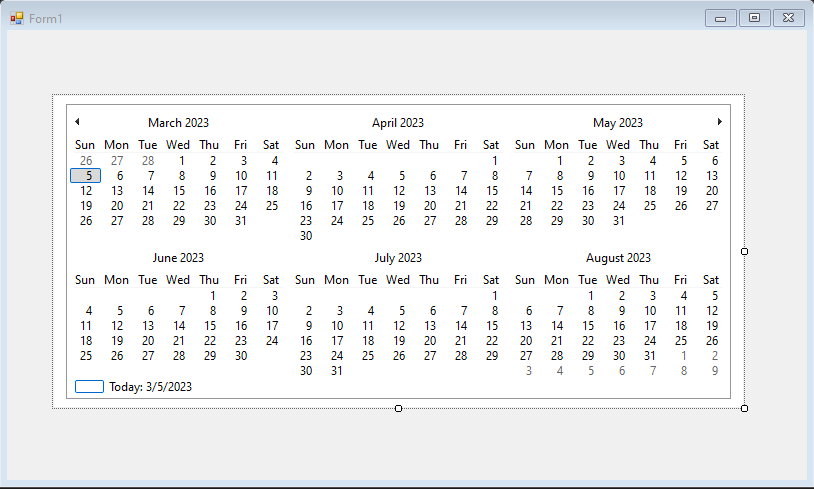
\includegraphics[scale=0.6]{gui.png}
\caption{GUI of application}
\label{GUI}
\end{figure}

Once the application is opened the user is greeted to a pleasant blue calendar displaying the current date. On the left is are the controls to change the background of the calendar and on the right are the controls to set an event.

\section{Project Timeline}
\begin{figure} [ht!]
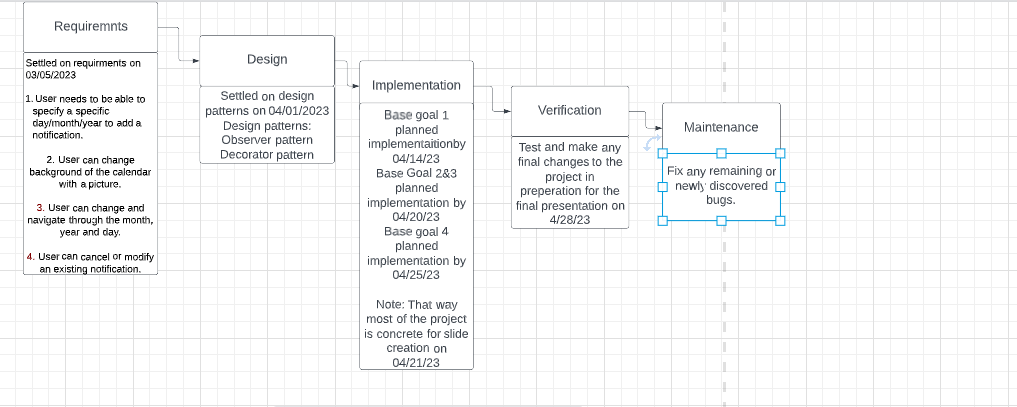
\includegraphics[scale=0.65]{Roadmap.png}
\caption{Project timeline}
\label{timeline}
\end{figure}

The above figure is the approximate timeline that our project followed. We followed the waterfall software development life cycle. Starting with requirements, we decided on what would define done for our project and what we would like to accomplish. Then we progressed to design, where we considered design patterns and the general structure of the program. Then came implementation, we encountered the most difficulties of the project in this phase. We eventually over came them and prevailed. Then we progressed to verification, this phase was shorter than planned as is common in waterfall. Now we are in the maintenance phase.

\section{Project Structure}
The way we designed the project so that where the user sees all their current events and notifications is clean. We tried implementing new windows for settings and events but could not get it working. We laid out all the functionality on the main window in a clean and strait forward way for the user. 

\subsection{UML Outline}
We chose the decorator pattern as we already found a calender object we could just decorate to help meet one of our base goals. We chose the observer pattern so that while the calender is not actively running the notifications can be checked to see if the set time has passed. Our concrete observers are the calendar blackout dates objects and the notification objects.
For example, see Figure \ref{UML of Calender Project}.

\begin{figure}[ht!]
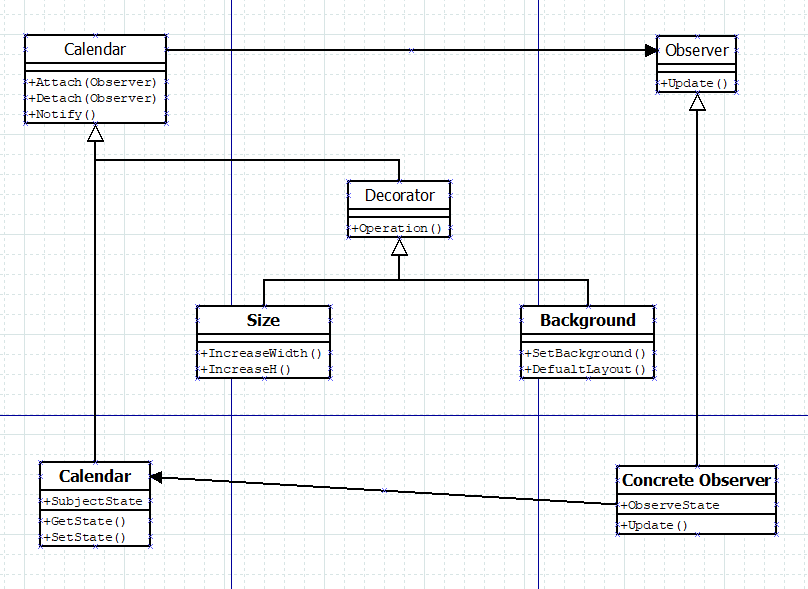
\includegraphics[scale=0.45]{Uml Format.png}
\caption{Uml outline of our Calender project}
\label{UML of Calender Project}
\end{figure}

\subsection{Design Patterns Used}
We are implementing the observer and decorator patterns. The decorator pattern to add new functionality to the calendar object we are using. The observer pattern to notify the user when a set event is happening. In regards to \ref{UML of Calender Project} the decorator pattern can be seen in the center of the figure and the observer can be seen around the outer edge. The two patterns both utilize the calendar object but they do not interfere with each other. 


\section{Results}
We implemented use cases 1, 2 and 3. The user can set the background of the calendar with an image using the images file path. The user can set a notification and remove a set notification. We did not finish implementing use case 4. Historic information and holidays are not in the current version of the application.


\subsection{Future Work}
We would like to build new features into our project in the future. We did not meet one of our base goals and would like to finish implementing that as we feel it is important to our project. We also want to expand our knowledge with C\# and push the boundary of what we thought was possible. One feature we wanted to implement was the exporting and importing from other calendar applications. However, if that does not come to fruition our project will be linked on our resume.



\begin{thebibliography}{1}

\bibitem{IEEEhowto:kopka}
H.~Kopka and P.~W. Daly, \emph{A Guide to \LaTeX}, 3rd~ed.\hskip 1em plus
  0.5em minus 0.4em\relax Harlow, England: Addison-Wesley, 1999.

\end{thebibliography}



\begin{IEEEbiography}{Michael Shell}
Biography text here.
\end{IEEEbiography}

% if you will not have a photo at all:
\begin{IEEEbiographynophoto}{John Doe}
Biography text here.
\end{IEEEbiographynophoto}

% insert where needed to balance the two columns on the last page with
% biographies
%\newpage

\begin{IEEEbiographynophoto}{Jane Doe}
Biography text here.
\end{IEEEbiographynophoto}





% that's all folks
\end{document}


